\documentclass[a4paper, 11pt]{article}
\usepackage{graphicx} % Required for inserting images
\usepackage{amsmath}
\usepackage{geometry}
\usepackage{hyperref}
\usepackage{setspace}
\usepackage{array}
\usepackage[usenames,dvipsnames]{xcolor}
\usepackage{colortbl} 
\usepackage{tabularray}
\usepackage[italian]{babel}
\definecolor{darkgreen}{RGB}{18,94,40}
\definecolor{lightgreen}{RGB}{179,255,179}
\definecolor{moregreen}{RGB}{153,255,143}
 \geometry{
 a4paper,
 left=25mm,
 right=25mm,
 top=20mm,
 bottom=20mm,
 }

\setlength{\parskip}{1em}
\setlength{\parindent}{0pt}

\begin{document}

\begin{minipage}{0.35\linewidth}
    
\includegraphics[width=\linewidth]{Logo_Universita_Padova.svg.png}
\end{minipage}\hfil
\begin{minipage}{0.55\linewidth}
\textbf{Università degli Studi di Padova} \\
Laurea in Informatica \\
Corso di Ingegneria del Software \\
Anno Accademico 2023/2024
\end{minipage}

\vspace{5mm}

\begin{minipage}{0.35\linewidth}
    
\includegraphics[width=\linewidth]{logo rotondo.jpg}
\end{minipage}\hfil
\begin{minipage}{0.55\linewidth}
\textbf{Gruppo:} SWEet16 \\
\textbf{Email:} 
\href{mailto:sweet16.unipd@gmail.com}{\nolinkurl{sweet16.unipd@gmail.com}}
\end{minipage}

\vspace{15mm}

\begin{center}
\begin{Huge}
        \textbf{Preventivo costi ed assunzione impegni} \\
        \vspace{4mm}
        
\end{Huge}

\vspace{20mm}

\begin{large}
\begin{spacing}{1.4}
\begin{tabular}{c c c}
   Redattori:  &  Alberto M. & \\
   Verificatori: & Iulius S. & Alex S. \\
   Amministratore: & Alberto C. & \\
   Destinatari: & T. Vardanega & R. Cardin \\  
   Versione: & 2.0.0 & 
\end{tabular}
\end{spacing}
\end{large}
\end{center}

\pagebreak

\begin{huge}
    \textbf{Registro delle modifiche}
\end{huge}
\vspace{5pt}

\begin{tblr}{
colspec={|X[1.5cm]|X[2cm]|X[2cm]|X[2.6cm]|X[6cm]|},
row{odd}={bg=white},
row{even}={bg=lightgray},
row{1}={bg=black,fg=white}
}
    Versione & Data & Autore & Ruolo & Descrizione \\
    \hline
    2.0.0 & 2023/11/06 & Alberto M. & Responsabile & Approvazione per rilascio \\
    \hline
    1.2.0 & 2023/11/06 & Bilal E. & Analista & Verifica documento \\
    \hline
    1.1.0 & 2023/11/06 & Alberto M. & Responsabile & Stesura sezione 3,6 \newline
    Modifica sezione 4,7 \\
    \hline
    1.0.0 & 2023/10/30 & Alberto M. & Responsabile & Approvazione per rilascio \\
    \hline
     0.4.0 & 2023/10/25 & Alex S. & Verificatore & Verifica documento \\
    \hline
    0.3.0 & 2023/10/24 & Alberto M. & Responsabile & Stesura sezioni 4,5,7 \\
    \hline
    0.2.0 & 2023/10/22 & Iulius S. & Verificatore & Verifica sezioni 1,2  \\
    \hline
     0.1.0   & 2023/10/22 & Alberto M. & Responsabile & Stesura sezioni 1,2 \\
     \hline
\end{tblr}

\pagebreak

\tableofcontents
\pagebreak

\section{Introduzione}

\subsection{Scopo del documento}

In questo documento viene riportato il preventivo per il progetto, andando ad analizzare singolarmente i vari ruoli e suddividendo le ore di lavoro dei vari componenti del gruppo.\\


Per riportare i nomi dei ruoli nelle tabelle, essi sono stati abbreviati come segue:
\begin{itemize}
    \item \textbf{Re:} Responsabile;
    \item \textbf{Am:} Amministratore;
    \item \textbf{An:} Analista;
    \item \textbf{Pg:} Progettista;
    \item \textbf{Pr:} Programmatore;
    \item \textbf{Vf:} Verificatore;
\end{itemize} 

\vspace{10pt}
\subsection{Riferimenti}
\begin{enumerate}
    \item Regolamento del Progetto Didattico , disponibile su  \url{https://www.math.unipd.it/~tullio/IS-1/2023/Dispense/PD2.pdf}
\end{enumerate}

\pagebreak

\section{Suddivisione dei ruoli}

La suddivisione oraria dei ruoli sarà così effettuata:
\begin{itemize}
    \item Ogni componente del gruppo dovrà ricoprire tutti i ruoli almeno una volta, in modo che tutti apprendano le responsabilità ed attività di ogni ruolo.

    \item Abbiamo deciso di suddividere equamente le ore dei vari ruoli per ogni componente del gruppo, per far si che ogni persona contribuisca allo stesso modo al progetto.
    
    \item Ogni componente del gruppo dovrà ricoprire non più di un ruolo alla volta.
\end{itemize}
\vspace{5pt}

\section{Analisi dei ruoli}
In questo paragrafo andremo ad analizzare singolarmente i vari ruoli di progetto, mostrando le motivazioni che hanno portato il gruppo alla suddivisione delle ore assegnate.

\subsection{Responsabile}
La figura del Responsabile garantisce il completamento del progetto in modo rapido, efficiente ed in linea con le aspettative del committente, verificando la corretta rotazione dei ruoli da parte dei componenti del gruppo. \\
Il Responsabile occupa un numero di ore inferiore alla media poiché, secondo la nostra analisi di progetto, necessita meno ore produttive per portare a termine i propri compiti rispetto ad altri ruoli, è inoltre il ruolo più economicamente dispendioso.

\subsection{Amministratore di sistema}

La figura dell'Amministratore di sistema garantisce e supervisiona il dominio informatico e tecnologico necessari per lo sviluppo e l'esecuzione del progetto. \\
Si occupa lui di decidere e mettere a disposizione le risorse utili al \textit{Way of Working} colletivo. \\
Anche l'Amministratore necessita di un numero di ore inferiore alla media perché utilizza meno tempo per completare i propri compiti.

\subsection{Analista}
Chi ricopre il ruolo di Analista è chiamato a ricoprire un ruolo fondamentale per l'analisi e la corretta comprensione dei problemi relativi al progetto. \\
Tuttavia sarà necessario solo durante determinate fasi di sviluppo del progetto, soprattutto all'inizio (in particolar modo nell'analisi dei requisiti), per questo abbiamo assegnato a questo ruolo un numero inferiore di ore rispetto agli altri ruoli.
\pagebreak
\subsection{Progettista}

Il Progettista è incaricato delle scelte realizzative per rendere possibile quanto emerso dal precedente lavoro degli analisti; si occupa della progettazione dell'architettura software identificando standard, strumenti e piattaforme da utilizzare. \\
Questa figura è un ruolo essenziale per garantire che il progetto sia ben strutturato, efficiente, sicuro e di facile comprensione per i suoi utilizzatori. \\
Alla luce della nostra analisi di progetto, riteniamo che la fase di progettazione necessiti di un buon quantitativo di ore.

\subsection{Programmatore}
Il Programmatore è la figura a cui vengono assegnate più ore per ruolo, questo perché andrà a ricoprire un ruolo chiave nello sviluppo del progetto; sarà colui che andrà a realizzare le scelte implementative dei progettisti e si occuperà della manutenzione del prodotto nel suo ciclo di vita. \\
Ritenendo che la fase di implementazione, per il capitolato scelto, sarà più dispendiosa in termini temporali rispetto al lavoro di analisti e progettisti, abbiamo deciso di assegnare al ruolo di programmatore un alto quantitativo di ore.

\subsection{Verificatore}
Il Verificatore andrà ad investire un ruolo primario all'interno del progetto, in quanto andrà a garantire la conformità e la correttezza del prodotto, nonché della sua documentazione. \\
Questo ruolo sarà presente durante tutto il ciclo di vita del progetto, soprattutto nella parte finale, in cui sarà essenziale garantire affidabilità e robustezza dei test del prodotto software. \\
Per questi motivi si è deciso di assegnare al ruolo di verificatore un monte ore notevole.

\pagebreak
\section{Impegni orari}

Ogni studente del gruppo \textbf{SWEet16} si impegna a lavorare al Progetto per un totale di 95 ore produttive.
Queste verranno suddivise equamente tra i ruoli a rotazione.

Si riporta il riepilogo della distribuzione oraria:


\begin{table}[h]
\begin{tblr}{
colspec={X[4cm]XXXXXXX},
row{odd}={bg=moregreen},
row{even}={bg=lightgreen},
row{1,8}={bg=darkgreen,fg=white}
}
    Nome & Re & Am & An & Pg & Pr & Vf & Totale \\
    
     Alberto Cinel & 9 & 10 & 9 & 13 & 28 & 26 & 95 \\
     
     Bilal El Moutaren & 9 & 10 & 9 & 13 & 28 & 26 & 95 \\
     
     Alberto Michelazzo & 9 & 10 & 9 & 13 & 28 & 26 & 95 \\
     
     Alex Scantamburlo & 9 & 10 & 9 & 13 & 28 & 26 & 95 \\
     
     Iulius Signorelli & 9 & 10 & 9 & 13 & 28 & 26 & 95 \\
     
     Giovanni Zuliani & 9 & 10 & 9 & 13 & 28 & 26 & 95 \\
     Totale & 54 & 60 & 54 & 78 & 168 & 156 & 570
     
\end{tblr}
\caption{Tabella contenente il riepilogo della distribuzione oraria}
    \label{Tabella:1}
\end{table}

\subsection{Schema a torta della distribuzione oraria dei ruoli}

\begin{figure}[h]
\centering
 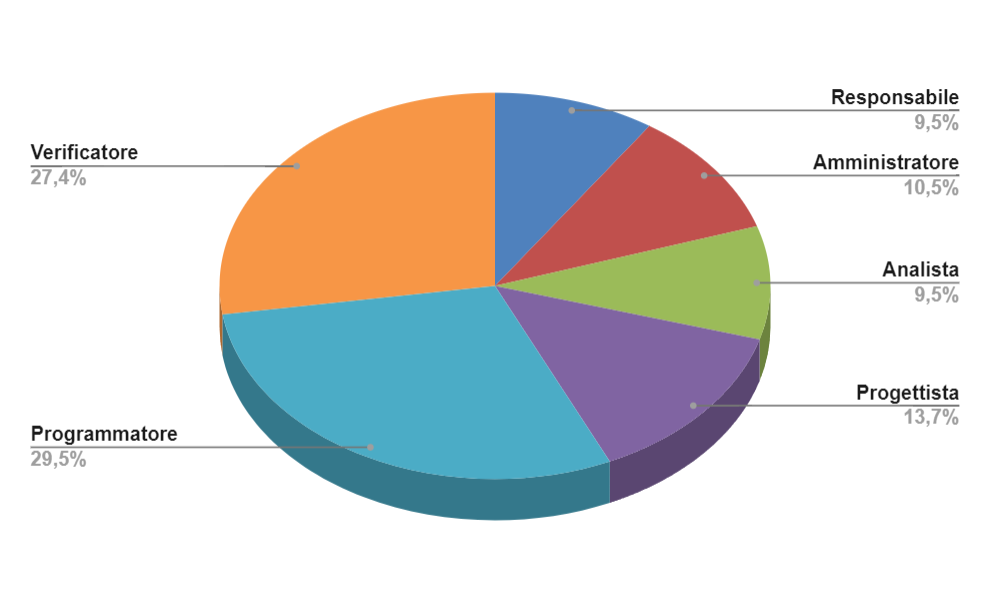
\includegraphics[width=\linewidth]{grafico a torta.png}
 \caption{Grafico a torta contenente la distribuzione oraria}
    \label{Immagine:1}
\end{figure}
\pagebreak

\section{Preventivo costi}
Si riporta il costo orario per ruolo, con conseguente costo totale:

\begin{table}[h]
\begin{tblr}{
colspec={X[4cm]XXXX},
row{odd}={bg=moregreen},
row{even}={bg=lightgreen},
row{1,8}={bg=darkgreen,fg=white}
}
    Ruolo & Ore (h) & Compenso orario (€/h) & Costo (€) & Peso(\%) \\
    Responsabile & 54 & 30,00 & 1620,00 & 14,80 \\
    Amministratore & 60 & 20,00 & 1200,00 & 10,93 \\
    Analista & 54 & 25,00 & 1350,00 & 12,30 \\
    Progettista & 78 & 25,00 & 1950,00 & 17,76 \\
    Programmatore & 168 & 15,00 & 2520,00 & 22,95 \\
    Verificatore & 156 & 15,00 & 2340,00 & 21,31 \\
    Totale & 570 &  & 10.980,00 & 100
\end{tblr}
\caption{Tabella contenente il riepilogo del prospetto economico}
    \label{Tabella:2}
\end{table}

\vspace{4pt}
Il costo finale del progetto ammonta a \textbf{10.980,00€} per 570 ore di lavoro totali, sulla base della pianificazione presentata e tenendo conto della fase preliminare di analisi. \\

\section{Rischi attesi}
\subsection{Utilizzo di nuove tecnologie}
Le tecnologie consigliate dall'azienda proponente utili per il completamento del capitolato sono conosciute solo in parte da alcuni membri del gruppo. \\
Il loro apprendimento potrà essere una difficoltà che andrà a rallentare l'inizio del progetto. \\
E' stato per questo pianificato un periodo iniziale dedicato allo studio delle tecnologie richieste per il completamento del progetto. \\
L'azienda \textit{Imola Informatica} si è inoltre resa disponibile per effettuare seminari di due/tre ore sulle tecnologie da utilizzare.

\subsection{Impegni ed imprevisti individuali}
Il nostro gruppo è formato da due studenti lavoratori a tempo pieno, più un'altra persona che lavora part-time. \\
Potrà quindi capitare che a volte non ci sarà modo di trovarsi tutti per gli incontri programmati in base agli impegni di ognuno. \\
Per risolvere questo problema abbiamo deciso di lavorare per la maggioranza del tempo in maniera asincrona, per poi trovarsi in maniera sincrona una o due volte a settimana, in base alle disponibilità di tutti. \\ \\
Sarà poi possibile che un membro del gruppo non porti a termine il lavoro assegnatogli a causa di imprevisti personali; la soluzione pensata per arginare questo potenziale problema si basa sulla trasparenza all'interno del gruppo, comunicando spesso e soprattutto quando si è impossibilitati a completare il proprio lavoro, in modo che questo possa essere diviso tra i restanti componenti del gruppo.

\subsection{Soddisfacimento delle aspettative del proponente}
Uno degli aspetti più importanti del progetto è poter garantire il soddisfacimento dei requisiti posti dall'azienda proponente; in caso di lacune nella comunicazione tra gruppo e proponente, ciò potrebbe non accadere. \\
Per mitigare questo problema si è pensato di effettuare frequenti incontri con il proponente, preparando anticipatamente domande rendicontate e versionate, per minimizzare i nostri dubbi ed il rischio di sbagliare.

\vspace{100pt}

\section{Promessa di consegna}
Il gruppo stima di consegnare il prodotto finito relativo al capitolato C3 "Easy Meal" proposto dall'azienda \textit{Imola Informatica} entro il 30/04/2024. \\ \\
Per un tempo totale di 25 settimane, così suddivise:
\begin{itemize}
    \item \textbf{7 settimane per lo sviluppo del \textit{PoC (Proof of Concept)}:} in questo periodo si acquisiranno competenze e conoscenze, e verrà portato a termine lo studio di fattibilità del progetto.
    \item \textbf{18 settimane per lo sviluppo del \textit{MVP (Minimum Viable Product)}:} in questa fase si svilupperà un prodotto funzionante e comprendente almeno tutti i requisiti minimi individuati dalla precedente analisi.
\end{itemize}

\end{document}

 